%\documentclass[a4paper, 11pt]{article}
\documentclass[UTF8]{ctexart}

\usepackage{amsmath}
\usepackage{graphicx}
\usepackage{geometry}
\usepackage{listings}
\usepackage{hyperref}

\usepackage{fontspec}
\setmonofont{Consolas}

\usepackage{xcolor}
\usepackage{enumerate}
\usepackage{array}
\usepackage{ulem}
\usepackage{titlesec} %自定义多级标题格式的宏包

\CTEXsetup[format={\large\bfseries}]{subsection}

\geometry{scale=0.8}
\linespread{1.5}
\title{	
\normalfont \normalsize
\textsc{School of Computer Science, Sun Yat-sen University} \\ [25pt] %textsc small capital letters
\rule{\textwidth}{0.5pt} \\[0.4cm] % Thin top horizontal rule
\huge  E04 Futoshiki Puzzle (Forward Checking) \\ % The assignment title
\rule{\textwidth}{2pt} \\[0.5cm] % Thick bottom horizontal rule
\author{19335016 HaoRan Chen}
\date{\normalsize \today} 
}

\begin{document}
\maketitle
\tableofcontents
\newpage

\section{Futoshiki}
Futoshiki is a board-based puzzle game, also known under the name Unequal. It is playable on a square board having a given fixed size (4 × 4 for example).

The purpose of the game is to discover the digits hidden inside the board’s cells; each cell is filled with a digit between 1 and the board’s size. On each row and column each digit appears exactly once; therefore, when revealed, the digits of the board form a so-called Latin square.

At the beginning of the game some digits might be revealed. The board might also contain some inequalities between the board cells; these inequalities must be respected and can be used as clues in order to discover the remaining hidden digits.

Each puzzle is guaranteed to have a solution and only one.

\begin{figure}
    \centering
    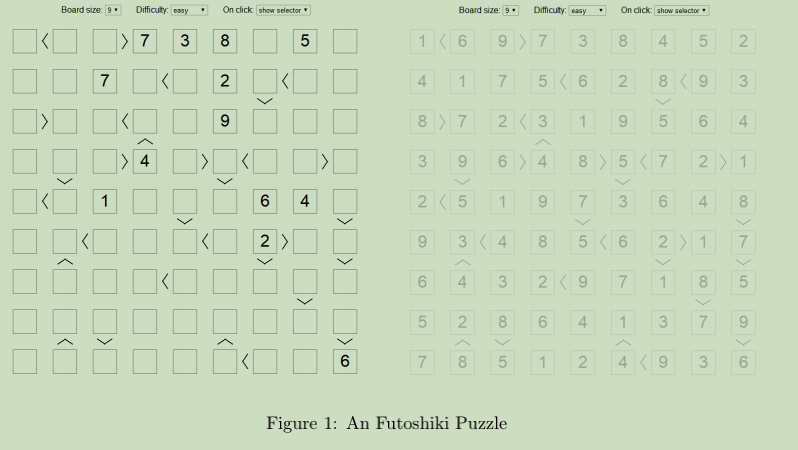
\includegraphics[width=15cm]{E04_Futoshi/figure1.png}
    \caption{Futoshiki}
    \label{fig:my_label}
\end{figure}

You can play this game online: http://www.futoshiki.org/.




\section{Tasks}
\begin{enumerate}

\item  Please solve the above Futoshiki puzzle ( Figure 1 ) with forward checking algorithm.

\item  Write the related codes and take a screenshot of the running results in the file named E04$\_$YourNumber.pdf, and send it to ai$\_$course2021@163.com.

\end{enumerate}

\section{Codes}
\begin{lstlisting}[language = C++, numbers=left,numberstyle=\tiny,keywordstyle=\color{blue!70},commentstyle=\color{red!50!green!50!blue!50},frame=shadowbox,rulesepcolor=\color{red!20!green!20!blue!20},basicstyle=\ttfamily]
#include <fstream>
#include <iostream>
#include <map>
#include <set>
#include <string>
#include <vector>
#include <ctime>
#define PII pair<int, int>
#define VVI vector<vector<int> >
#define VVSI vector<vector<set<int> > >
using namespace std;
const int SIZE=9;
//DWO: Domain Wipe Out,表示该节点(变量)的值域Domain已经为空。
class Futoshiki{
    public:
    VVI puzzle;
    //int puzzle[9][9];
    vector<pair<PII, PII>> less_constraints;
    Futoshiki(){
        puzzle = {{0, 0, 0, 7, 3, 8, 0, 5, 0},
                  {0, 0, 7, 0, 0, 2, 0, 0, 0},
                  {0, 0, 0, 0, 0, 9, 0, 0, 0},
                  {0, 0, 0, 4, 0, 0, 0, 0, 0},
                  {0, 0, 1, 0, 0, 0, 6, 4, 0},
                  {0, 0, 0, 0, 0, 0, 2, 0, 0},
                  {0, 0, 0, 0, 0, 0, 0, 0, 0},
                  {0, 0, 0, 0, 0, 0, 0, 0, 0},
                  {0, 0, 0, 0, 0, 0, 0, 0, 6}};
        
        add(0, 0, 0, 1);	add(0, 3, 0, 2);
        add(1, 3, 1, 4);	add(1, 6, 1, 7);
        add(2, 6, 1, 6);	add(2, 1, 2, 0);
        add(2, 2, 2, 3);	add(2, 3, 3, 3);
        add(3, 3, 3, 2);	add(3, 5, 3, 4);
        add(3, 5, 3, 6);	add(3, 8, 3, 7);
        add(4, 1, 3, 1);	add(4, 5, 3, 5);
        add(4, 0, 4, 1);	add(5, 4, 4, 4);
        add(5, 8, 4, 8);	add(5, 1, 5, 2);
        add(5, 4, 5, 5);	add(5, 7, 5, 6);
        add(5, 1, 6, 1);	add(6, 6, 5, 6);
        add(6, 8, 5, 8);	add(6, 3, 6, 4);
        add(7, 7, 6, 7);	add(7, 1, 8, 1);
        add(8, 2, 7, 2);	add(7, 5, 8, 5);
        add(8, 8, 7, 8);	add(8, 5, 8, 6);
    }
    //计算总可行数
    int domainCount(const VVSI& domains) {
        int count = 0;
        for(int i = 0; i < SIZE; i++) for(int j = 0; j < SIZE; j++)
        count += domains[i][j].size();
        return count;
    }
    
    void add(int x, int y, int x1, int y1){
        less_constraints.push_back({{x, y}, {x1, y1}});
    }
    
    bool isSolved(){
        for(int i=0; i<SIZE; i++) for(int j=0; j<SIZE; j++) 
        if(puzzle[i][j]==0) return false;
        return true;
    }
    
    //初始化每个格子的可行域
    VVSI makeDomains(){
        VVSI domains(SIZE, vector<set<int> >(SIZE, set<int>()));
        for(int i = 0; i < SIZE; i++) for(int j = 0; j < SIZE; j++){
            if(puzzle[i][j]==0) for(int k = 0; k < SIZE; k++) 
                domains[i][j].insert(k + 1);
            else domains[i][j].insert(puzzle[i][j]);
        }
        
        for(int i = 0; i < SIZE; i++) for(int j = 0; j < SIZE; j++){
            if(puzzle[i][j]!=0){
                for(int ii = 0; ii < SIZE; ii++) if(ii != i) 
                    domains[ii][j].erase(puzzle[i][j]);
                for(int jj = 0; jj < SIZE; jj++) if(jj != j) 
                    domains[i][jj].erase(puzzle[i][j]);
            }
        }
        //清除不符合约束条件的数
        for (int i = 0; i < less_constraints.size(); i++) {
            PII sp = less_constraints[i].first;
            PII lp = less_constraints[i].second;
            if (puzzle[lp.first][lp.second] != 0) { 
                for (int k = puzzle[lp.first][lp.second]; k <= SIZE; k++) 
                    domains[sp.first][sp.second].erase(k);
            }
            else {
                int minimum = *domains[sp.first][sp.second].begin();
                domains[lp.first][lp.second].erase(minimum);
            }
            if (puzzle[sp.first][sp.second] != 0) {
                for (int k = 1; k <= puzzle[sp.first][sp.second]; k++) {
                    domains[lp.first][lp.second].erase(k);
                }
            }
            else {
                int minimum = *domains[lp.first][lp.second].rbegin();//取最后元素
                domains[sp.first][sp.second].erase(minimum);
            }
        }
        return domains;
    }
    
    //在每次迭代中使用MRV函数选择一个位置,并在其域中分配一个值。
    //然后通过删除一些与赋值冲突的值来更新一些格子的域。
    VVSI updateDomains(VVSI domains, const PII& pos) {
        // 检查列
        for (int i = 0; i < SIZE; i++) {
            if (i == pos.first) continue;
            else if (puzzle[i][pos.second] == puzzle[pos.first][pos.second]) 
                return VVSI();		// DWO
            else {
                domains[i][pos.second].erase(puzzle[pos.first][pos.second]);
                if (domains[i][pos.second].size() == 0) return VVSI(); // DWO
            }
        }
        
        // 检查行
        for (int j = 0; j < SIZE; j++) {
            if (j == pos.second) continue;
            else if (puzzle[pos.first][j] == puzzle[pos.first][pos.second]) {
                return VVSI();  		// DWO
            } 
            else {
                domains[pos.first][j].erase(puzzle[pos.first][pos.second]);
                if (domains[pos.first][j].size() == 0) {
                    return VVSI();  	// DWO
                }
            }
        }
        
        // 检查约束条件
        for (int i = 0; i < less_constraints.size(); i++) {
            PII sp = less_constraints[i].first;
            PII lp = less_constraints[i].second;
            if (pos == lp) {
                for (int k = puzzle[pos.first][pos.second]; k <= SIZE; k++) {
                    domains[sp.first][sp.second].erase(k);
                    if (puzzle[sp.first][sp.second] == 0 && 
                domains[sp.first][sp.second].size() == 0) 
                        return VVSI();  // DWO
                    
                }
            } 
            else if (pos == sp) {
                for (int k = 1; k <= puzzle[pos.first][pos.second]; k++) {
                    domains[lp.first][lp.second].erase(k);
                    if (puzzle[lp.first][lp.second] == 0 && 
                domains[lp.first][lp.second].size() == 0) 
                        return VVSI();  // DWO
                    
                }
            }
        }
        return domains;
    }
    
    //选择可行域最小的格子并返回其位置, minimum remaining values (MRV)
    PII MRV(const VVSI& domains) {
        int val = 114514;  
        PII pos = make_pair(-1, -1);
        for (int i = 0; i < SIZE; i++) {
            for (int j = 0; j < SIZE; j++) {
                if (puzzle[i][j] == 0 && domains[i][j].size() < val) {
                    val = domains[i][j].size();
                    pos = make_pair(i, j);
                }
            }
        }
        return pos;
    }
    
    VVI ForwardChecking(const VVSI& domains) {
        if (isSolved()) return puzzle;
        PII pos = MRV(domains);
        for (auto p = domains[pos.first][pos.second].begin(); 
                  p != domains[pos.first][pos.second].end(); p++) {
            puzzle[pos.first][pos.second] = *p;
            auto temp_domains = updateDomains(domains, pos);
            if (temp_domains.size() != 0) { 
                VVI res = ForwardChecking(temp_domains);
                if (res.size() != 0) return res;
            }
        }
        
        puzzle[pos.first][pos.second] = 0;
        return VVI();  
    }
    
    void print(){
        for(int i = 0; i < SIZE; i++){
            for(int j = 0; j < SIZE; j++) printf("%d ",puzzle[i][j]);
            printf("\n");
        }
        puts("======================");
    }
};
int main(){
    clock_t start, end;
    Futoshiki game;
    game.print();
    VVSI domains = game.makeDomains();
    
    start=clock();
    game.ForwardChecking(domains);
    end=clock();
    
    game.print();
    printf("\ntime is %lf s\n",((double)end-start)/CLOCKS_PER_SEC);
    return 0;
}
\end{lstlisting}
\newpage
\section{Results}

\begin{figure}[!h]
    \centering
    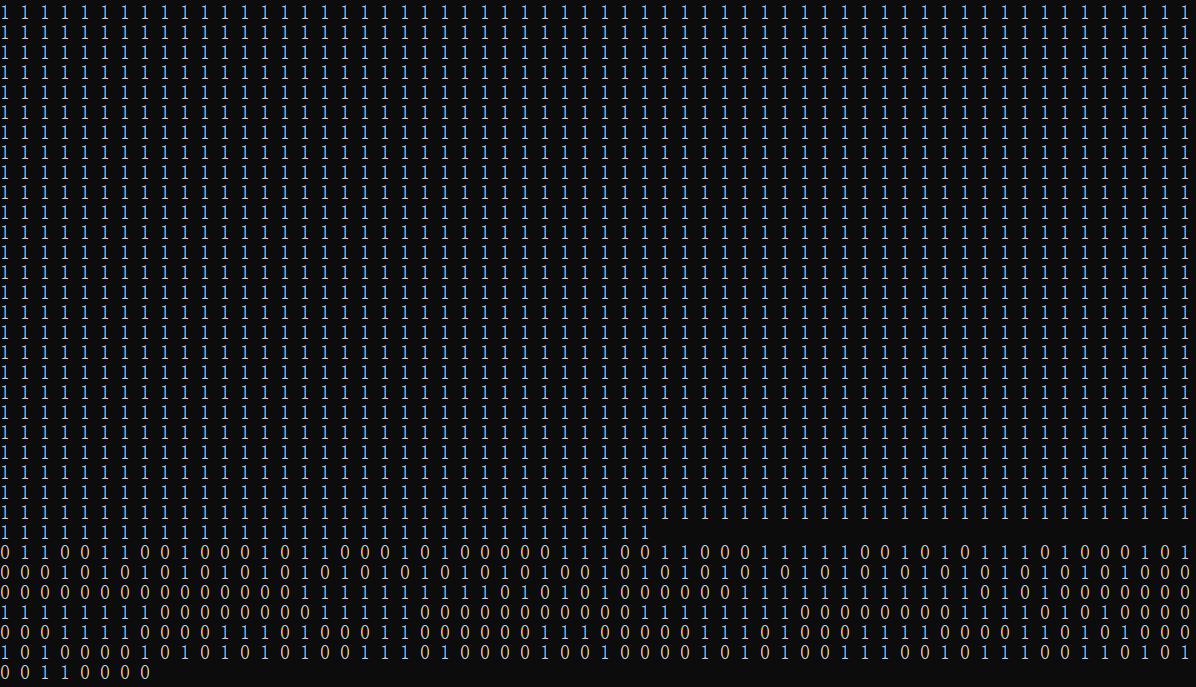
\includegraphics[width=0.8\textwidth]{res.bmp}
    %\caption{}
\end{figure}

其中, 左边为原back tracking算法的check函数运行结果,右边为本函数运行结果,可见相对于传统BackTracking算法,ForwardChecking运行速度有较大提升.
%\clearpage
%\bibliography{E:/Papers/LiuLab}
%\bibliographystyle{apalike}
\end{document} 
%%% Local Variables:
%%% mode: latex
%%% TeX-master: t
%%% End:

